\chapter{Angriffsmöglichkeiten}
\label{chap:kapitel2}
\nocite{WikipediaDoS}

\section{HTTP slow POST}

Diese Möglichkeit eines Angriffs versucht die maximale Anzahl an möglichen Verbindungen eines Servers auszuschöpfen, indem ein legitimer HTTP POST Request an den Server gesendet wird. Die Größe des Request wird dabei auf einen sehr hohen Wert gesetzt und die Übertragungsgeschwindigkeit sehr gering gewählt, sodass es ewig dauert den gesamten Request zu empfangen. Nun baut man einfach sehr viele solche Verbindungen auf, bis der Server irgendwann keine neuen Verbindungen mehr zulässt und der Dienst für legitime Nutzer nicht mehr erreichbar wrid.

\section{Ping of Death}

Der Ping of Death ist eine Möglichkeit, einen Fehler beim Zusammenbauen von empfangenen IP Nachrichten auszunutzen. Dieser Fehler führt dann zu einem Überlauf bei einem Speicher im angegriffenen System, welcher verschiedene schwerwiegende Folgen mit sich bringen kann, die im Normalfall einen Ausfall des Servers auslösen. Der Ping of Death konnte vor allem in frühen Implementierungen des TCP/IP Protokolls ausgenutzt werden und betraf damit viele Systeme, wie Windows und UNIX.

\section{Smurf Angriff}

Ein Smurf Angriff macht sich eine Eigenschaft von falsch konfigurierten Routern zunutze, indem eine Nachricht mit veränderter Quelladresse an einen Router geschickt wird. Die Zieladresse ist hierbei die Broadcast Adresse des entsprechenden Netzwerks. Man nimmt nun an, dass alle Endgeräte innerhalb des Netzwerks, welche die Nachricht erhalten, eine Antwort an den Sender schicken. Da man allerdings die Quelladresse des gesendeten Pakets zu dem eigentlichen Ziel des Angriffs geändert hat gehen die Antworten auf den Broadcast nicht an den Angreifer sondern an das Ziel des Angriffs. Der Nachteil dieser Methode ist der, dass normalerweise Router so eingestellt sind, dass sie nicht auf Broadcasts von außerhalb des Netzwerks reagieren.

\section{SYN Flood}

Eine SYN Flood benutzt den TCP three-way handshake um die maximale Anzahl an verfügbarer Verbindungen eines Servers auszuschöpfen. Bei einem normalen TCP three-way handshake wird erst eine SYN Nachricht von einem Client an den Server geschickt. Nachdem der Server diese SYN Nachricht empfangen hat antwortet dieser mit einer SYN-ACK Nachricht und wartet darauf, dass der Client mit einem ACK antwortet. Bei einem SYN Flood Angriff wird nun entweder einfach kein ACK geschickt oder man verändert die Senderadresse der ersten SYN Nachricht, sodass der Server seine SYN-ACK Nachricht einem unbeteiligten Dritten schickt, welcher die Nachricht ignoriert. Die Folge ist dann, dass der Server auf eine Nachricht wartet, welche nie gesendet wird und damit eine Verbindung verbraucht. Schickt man nun ausreichend SYN Nachrichten an den Server wird dieser irgendwann keine neuen Verbindungen mehr akzeptieren und ein legitimer Benutzer kann sich auch nicht mehr verbinden.

\begin{figure}[h]
		\centering
		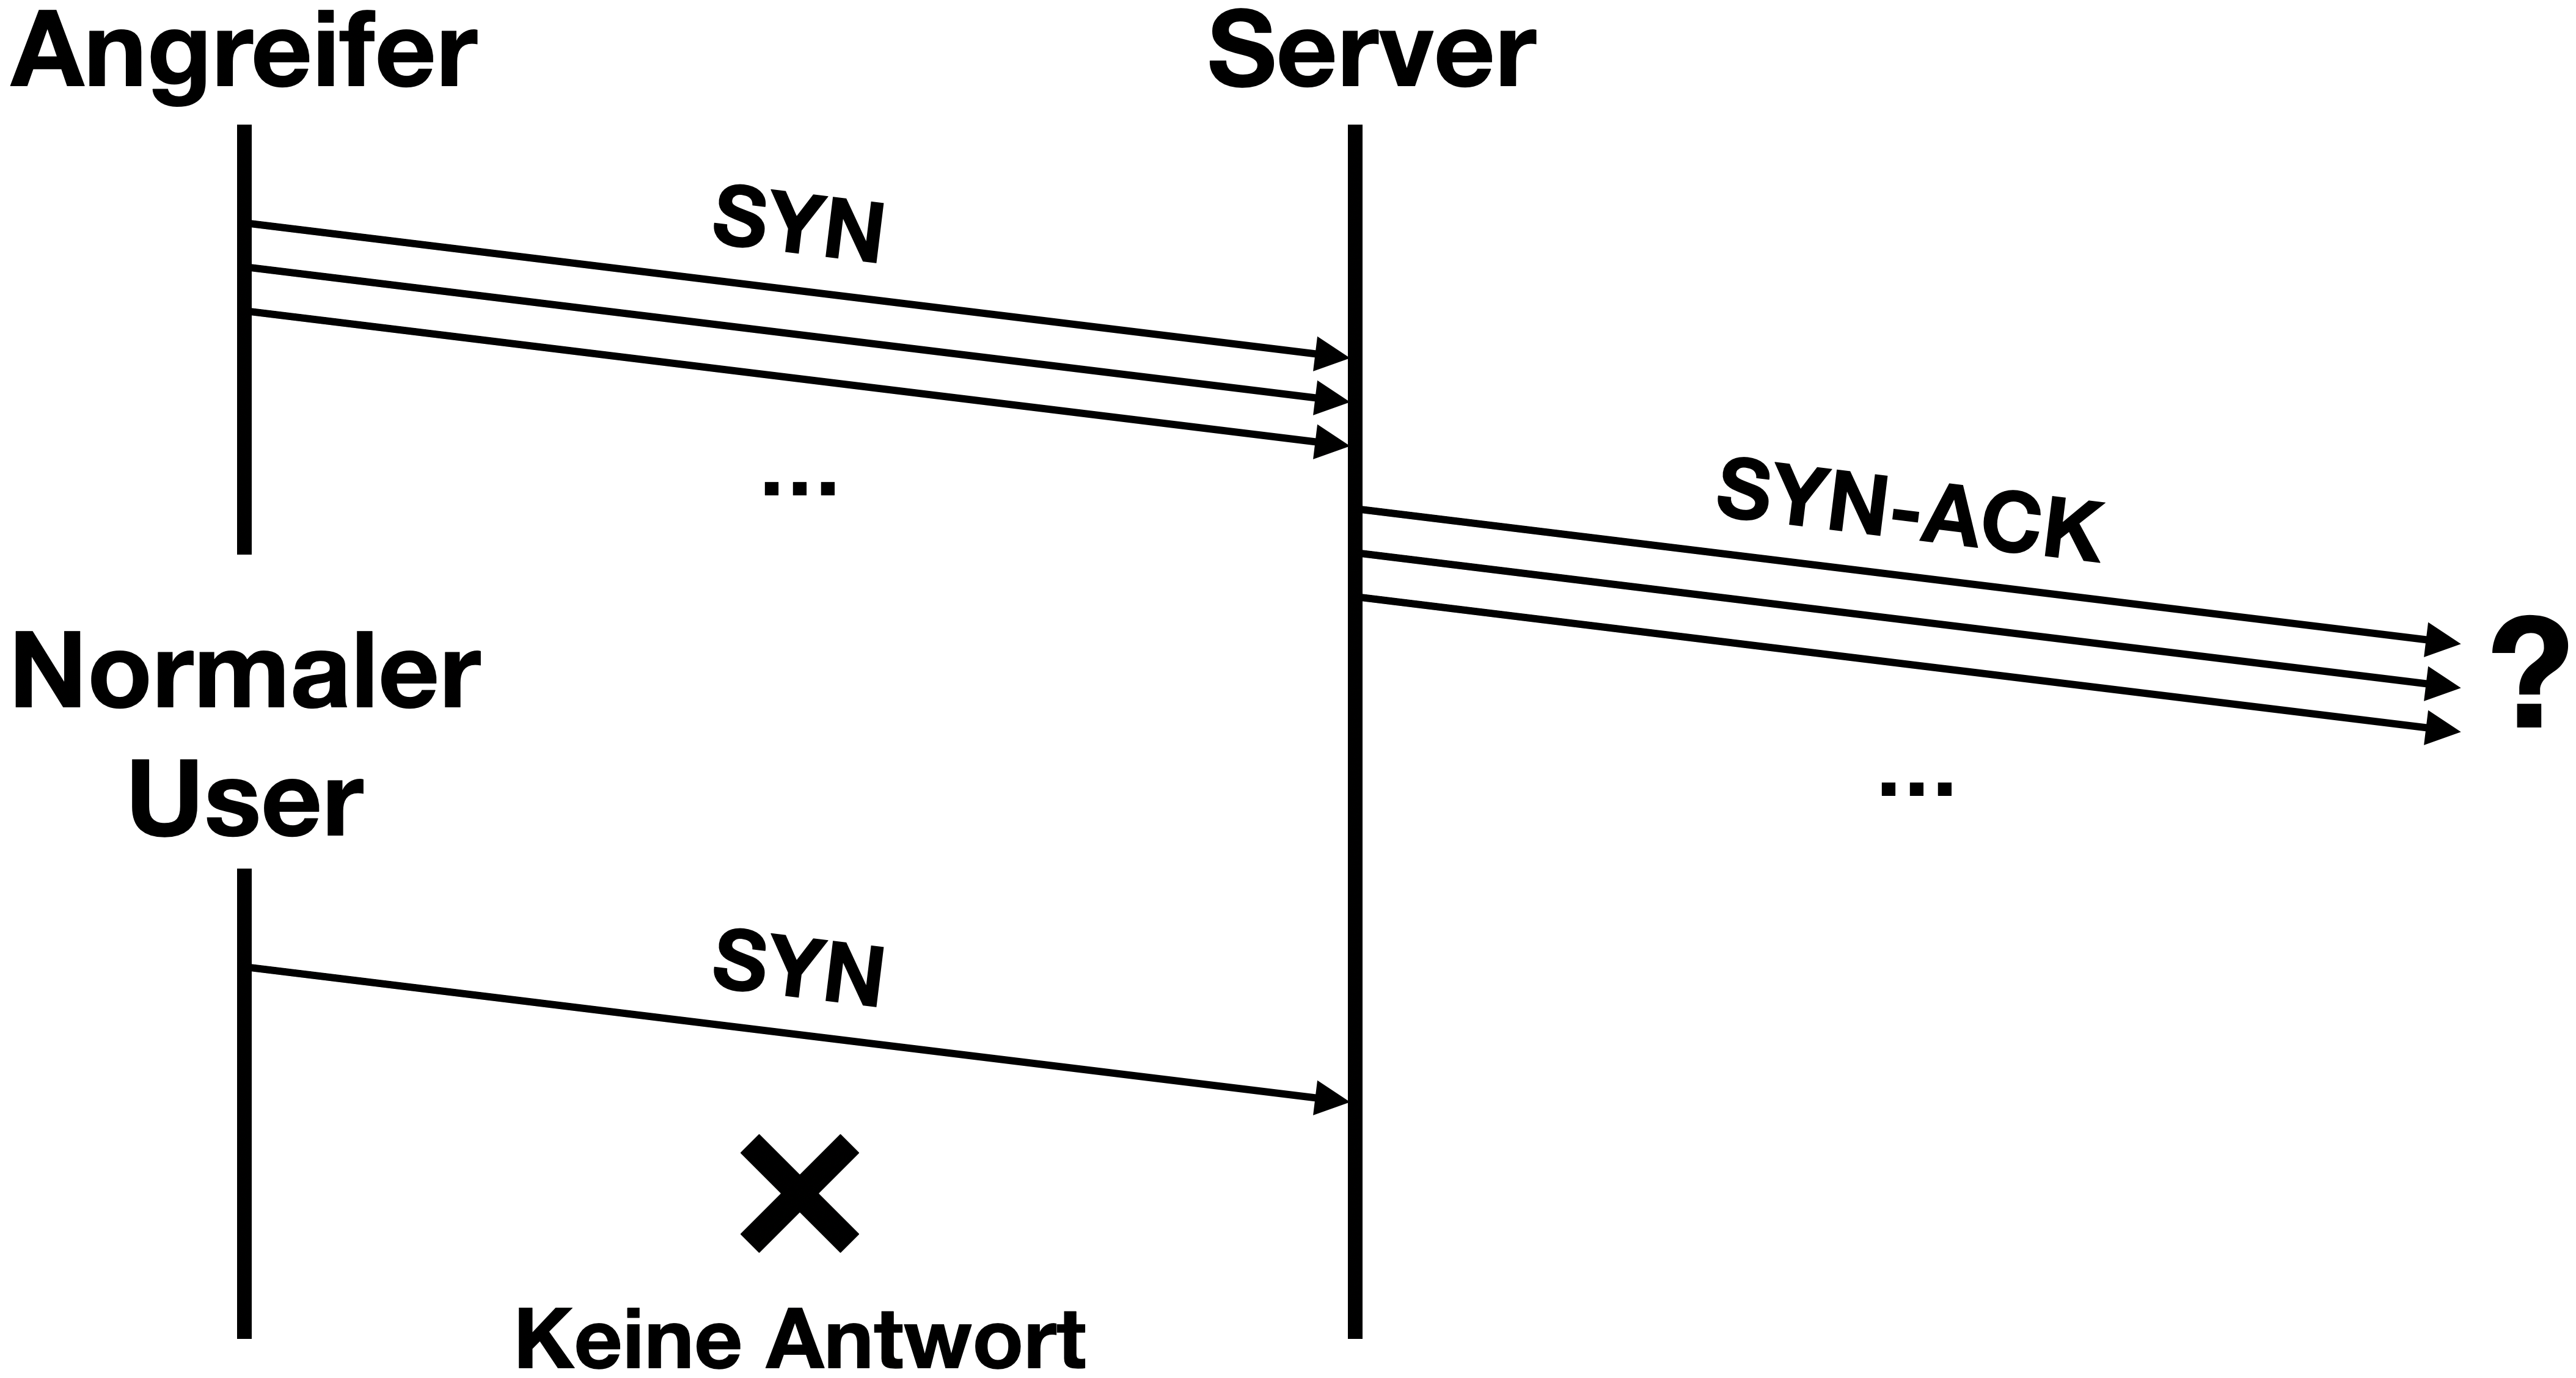
\includegraphics[width=\textwidth, center]{kapitel2/synflood}
		\caption[SYN-Flooding]{Prinzipieller Ablauf eines SYN-Flood Angriffs}
		\label{img:synflood}
\end{figure}

\section{Amplification}

Diese Angriffsmethode versucht die Bandbreite des Angegriffenen auszuschöpfen. Dazu werden öffentliche Server verwendet, um zu erreichen, dass mehr Daten beim Ziel des Angriffs ankommen, als vom Angreifer geschickt wurden. Um dies zu erreichen schickt man Anfragen an beispielsweise DNS Server und fordert von diesen eine möglichst große Antwort an. Damit diese Antwort dann beim Ziel des Angriffs ankommt wird die Sendeadresse der  Anfrage zur IP des Ziels geändert. Somit erhält der Zielserver eine sehr große Menge an Daten, welche bei einem erfolgreichen Angriff ausreichen um die Internetverbindung des Ziels völlig auszulasten und damit den Zugriff auf den Zielserver für legitime Nutzer zu erschweren oder ganz zu unterbinden. Wenn man DNS Server zum Vergrößern der Nachrichten verwendet kann man einen Verstärkungsfaktor von bis zu 179 erreichen. Diese Angriffsmöglichkeit hat den Vorteil, dass der Angreifer selbst keine extreme Bandbreite benötigt, um einen großen Einfluss beim Ziel zu erreichen.

\section{TTL Expire}

Dieser Angriff versucht Router zu überlasten. Er macht sich die Eigenschaft zu nutze, dass ein Router zum Verwerfen einer ankommenden Nachricht deutlich mehr Zeit braucht, als für das einfache Weiterleiten. Das kommt daher, dass der Router dazu verpflichtet ist beim Ablaufen der TTL eine ICMP time exceeded Nachricht zu generieren und zu versenden. Wenn zu viele solcher Nachrichten generiert werden müssen kann das die CPU des Routers auslasten und damit das Weiterleiten legitimer Nachrichten verzögern oder blockieren. Um das in einem Angriff auszunutzen muss man lediglich die Anzahl Hops zum Zielrouter ermitteln und anschließend sehr viele Nachricht mit entsprechend gesetzter TTL schicken.